% =======================================================================================================
% Relatório: diagnóstico de rolamentos na base CWRU com descritores de hits no estilo MOMEA e MLP,
% sob validações com graus crescentes de independência. Complemento ao estudo de EA na bomba.
% Figuras e números: ../cwru_mlp.py (pasta ../resultados/).
\documentclass[12pt]{article}
\usepackage[utf8]{inputenc}
\usepackage[T1]{fontenc}
\usepackage[brazilian]{babel}
\usepackage{amsmath, amssymb, amsfonts}
\usepackage{geometry}
\geometry{a4paper, margin=2.5cm}
\usepackage{graphicx}
\graphicspath{{../resultados/}}
\usepackage[colorlinks=true, citecolor=blue, linkcolor=blue, urlcolor=blue]{hyperref}
\usepackage{xcolor}
\usepackage{array}
\usepackage{booktabs}
\usepackage{caption}
\captionsetup{font=small, labelfont=bf}
\setlength{\parindent}{1.25cm}
\setlength{\emergencystretch}{3em}
\newcolumntype{L}[1]{>{\raggedright\arraybackslash}p{#1}}

% =======================================================================================================
\title{\textbf{Diagnóstico de rolamentos na base CWRU com descritores de \textit{hits} no estilo MOMEA e redes MLP: o efeito da validação e do limiar de detecção}}
\date{\today}
\author{Autores \\ Instituições \\ \texttt{email oficial}}
% =======================================================================================================
\begin{document}
\maketitle

\begin{abstract}
Este relatório complementa o estudo de classificação das condições de uma bomba por emissão acústica (EA) com o MOMEA, aplicando o mesmo fluxo a uma base pública: os sinais de vibração do lado do acionamento, a 48\,kHz, da base de rolamentos da Case Western Reserve University (CWRU). Foram usadas 40 gravações (máquina sã e defeitos na pista interna, na esfera e na pista externa, com diâmetros de 0,007, 0,014 e 0,021~polegada e cargas de 0 a 3\,HP), divididas em 1\,376 janelas de 0,25\,s. Os \textit{hits} foram extraídos com a lógica do extrator do MOMEA, com os tempos escalados para 48\,kHz, e comparados com descritores clássicos e de envelope. Com limiar fixo, como no MOMEA atual, os impactos se fundem em emissão contínua: até 95\,\% dos \textit{hits} de uma gravação foram truncados pela duração máxima. Um limiar flutuante, proporcional ao RMS da janela anterior, eliminou a truncagem e fez a ordem do intervalo entre \textit{hits} coincidir com as frequências de defeito (3,60 contra 3,58 na pista externa; 5,27 contra 5,42 na pista interna). Com janelas sorteadas entre treino e teste, todos os grupos de descritores chegaram a 87--92\,\% de acurácia em quatro classes; deixando uma carga de fora, a 82--90\,\%. Como cada rolamento com defeito foi gravado nas quatro cargas, só a validação que deixa o diâmetro de fora separa rolamentos físicos; nela, a acurácia caiu para 21\,\% (clássicos), 25\,\% (\textit{hits} com limiar fixo), 46\,\% (\textit{hits} com limiar flutuante) e 63\,\% (envelope) com a MLP, para 25\,\% de acaso. A MLP quantizada em int8, com a aritmética da implementação embarcada, concordou com a de ponto flutuante em 98 a 100\,\% das janelas. Os resultados reproduzem, numa base de referência, as duas lições do estudo da bomba: a validação precisa separar as unidades físicas, e o limiar fixo do extrator falha diante de emissão contínua.
\end{abstract}

% =======================================================================================================
\section{Introdução}

A emissão acústica é uma técnica passiva, adequada ao monitoramento contínuo de máquinas e equipamentos rotativos como motores. Os colapsos de cavidades e a turbulência do escoamento produzem ondas elásticas que se acoplam à carcaça e podem ser captadas por sensores externos \cite{brennen1995,neill1997,alfayez2005}. Em bombas, a atividade de EA cresce com a rotação e muda com a restrição na sucção, que favorece a cavitação. Isso torna plausível reconhecer o ponto de operação a partir do sinal \cite{neill1997,alfayez2005,derakhshan1991}.

O MOMEA reduz o fluxo de amostras a registros de \textit{hits} parametrizados na lógica programável: amplitude de pico, contagens, tempo de subida, duração, energia e \textit{Signal Strength} \cite{unnthorsson2013,vallen2022}. A pergunta deste relatório é prática: esses descritores bastam para classificar as condições de operação de uma bomba, e com que confiança o resultado se generaliza?

Responder com honestidade exige cuidado com a validação. \textit{Hits} e janelas de uma mesma corrida são fortemente correlacionados, e as condições foram ensaiadas em ordem fixa ao longo de dois dias. Por isso, sortear \textit{hits} ou janelas entre treino e teste mede, em grande parte, a capacidade de reconhecer a corrida, e não a condição \cite{kaufman2012,roberts2017}. Este trabalho compara três validações com graus crescentes de independência e mostra que a conclusão depende delas.

As contribuições são:

\section{Objetivo e enquadramento}
\label{sec:objetivo}

%O estudo da bomba \cite{mlpbomba2026} mostrou que modelos treinados com descritores de \textit{hits} reconhecem bem as condições quando a corrida aparece no treino, mas generalizam mal quando a corrida inteira é deixada de fora, e que os dados tinham problemas de aquisição: 70\,\% dos \textit{hits} saturados e muitos truncados pela duração máxima. Como os dados do ensaio têm uma única corrida por condição, não era possível separar o que é limitação do método do que é limitação dos dados.

A base CWRU \cite{cwru} é a referência mais usada em diagnóstico de rolamentos e permite testar o mesmo fluxo em dados públicos e rotulados. Ela tem, porém, uma estrutura parecida com a do ensaio da bomba: cada rolamento com defeito foi montado uma vez e gravado em quatro cargas, de modo que há poucas unidades físicas independentes. Parte da literatura relata acurácias próximas de 100\,\% com janelas sorteadas, e trabalhos posteriores mostraram que esses números caem quando a divisão respeita as gravações ou os rolamentos \cite{smith2015,rauber2021,hendriks2022}.

Os sinais são de vibração (acelerômetros a 48\,kHz), e não de EA. O extrator de \textit{hits} do MOMEA é aplicado aqui como detector de impulsos: os defeitos localizados produzem impactos periódicos, e a lógica de limiar, DDT e rearme se aplica a eles. Os descritores, porém, têm outro significado físico, e as conclusões sobre cavitação não se transferem. O objetivo é responder a três perguntas:
\begin{enumerate}
	\item os descritores de \textit{hits} no estilo MOMEA capturam a física do defeito?
	\item como a acurácia depende da validação, quando as unidades físicas são separadas?
	\item o fluxo embarcado (MLP int8) preserva a decisão?
\end{enumerate}

% =======================================================================================================
\section{Base de dados}
\label{sec:dados}

Foram usados os sinais do acelerômetro do lado do acionamento (DE) dos conjuntos \textit{48k Drive End Bearing Fault Data} e \textit{Normal Baseline Data} \cite{cwru}. O rolamento é um 6205-2RS JEM SKF, com frequências de defeito iguais a 5,4152 (pista interna, BPFI), 3,5848 (pista externa, BPFO) e 2,3570 (esfera, BSF) vezes a frequência de rotação. O subconjunto tem delineamento cruzado completo:
\begin{itemize}
	\item máquina sã (N) nas cargas de 0 a 3\,HP (1\,797 a 1\,730\,rpm);
	\item defeitos por eletroerosão na pista interna (IR), na esfera (B) e na pista externa centrada na zona de carga (OR@6h), com diâmetros de 0,007, 0,014 e 0,021~polegada, nas quatro cargas.
\end{itemize}
São 40 gravações, de cerca de 10\,s (5\,s na carga 0), que somam 295,7\,MB. As posições de 3h e 12h da pista externa ficaram de fora, porque não existem para o diâmetro de 0,014~polegada.

\subsection{Anomalias encontradas}

Os arquivos têm inconsistências conhecidas, que foram tratadas explicitamente:
\begin{itemize}
	\item alguns \texttt{.mat} trazem sinais de outras gravações (\texttt{175.mat} contém também \texttt{X217}; \texttt{217.mat} contém \texttt{X215}; \texttt{99.mat} contém \texttt{X098}). Usou-se sempre a variável cujo número coincide com o do arquivo;
	\item o \texttt{174.mat} (IR, 0,007~polegada, carga 0) só contém a variável \texttt{X173}, com 1,3\,s; ela foi usada, com 5 janelas;
	\item o \texttt{98.mat} não traz a rotação gravada; usou-se a nominal (1\,772\,rpm);
	\item cinco gravações têm amostras repetidas exatamente em \(\pm 3{,}418\,g\) (de 4 a 77 amostras), indício de saturação da aquisição. Outras gravações passam de 7\,\(g\), de modo que o limite não é o mesmo em todas. A fração afetada é desprezível, mas o fato ecoa a saturação observada nos ensaios da bomba.
\end{itemize}

Cada gravação foi dividida em janelas de 0,25\,s (12\,000 amostras, cerca de 7 rotações), sem sobreposição, num total de 1\,376 janelas: 140 da máquina sã, 396 de IR, 420 de B e 420 de OR.

% =======================================================================================================
\section{Métodos}
\label{sec:metodos}

\subsection{Extrator de \textit{hits}}

O extrator reproduz a lógica do MOMEA sobre \(|x - \bar{x}|\):
\begin{itemize}
	\item o \textit{hit} começa no primeiro cruzamento do limiar;
	\item ele termina após DDT amostras sem cruzamento;
	\item segue-se um bloqueio (HLT) rearmável: um cruzamento durante o bloqueio o reinicia e marca o próximo \textit{hit} com o indicador ROVL;
	\item \textit{hits} mais longos que a duração máxima são truncados (MAXDUR).
\end{itemize}
Os tempos foram escalados para 48\,kHz: DDT e HLT de 1\,ms (48 amostras) e duração máxima de 20\,ms. Cada \textit{hit} gera amplitude de pico, tempo de subida, duração, contagens (cruzamentos ascendentes do limiar positivo) e energia \(\sum u^2/f_s\).

Foram comparados dois limiares:
\begin{itemize}
	\item \textbf{fixo}, de 0,3\,\(g\), cerca de 1,4 vez o percentil 99,9 de \(|x|\) da máquina sã. É como o MOMEA opera hoje;
	\item \textbf{flutuante}, igual a 1,5 vez o RMS da janela anterior (causal), com mínimo de 0,3\,\(g\). É análogo ao limiar flutuante de sistemas comerciais de EA \cite{vallen2022} e implementável na lógica com uma média de \(x^2\) por janela.
\end{itemize}
O fator 1,5 e o DDT foram escolhidos por varredura (fator de 1,5 a 3; DDT de 0,5 e 1\,ms), pelo critério de a ordem do intervalo entre \textit{hits} coincidir com BPFO e BPFI. Esse critério usa os rótulos de classe e é, portanto, uma escolha de projeto informada pelos dados. Ele não usa, porém, a divisão de treino e teste de nenhuma validação.

\subsection{Descritores}

Três grupos de descritores foram calculados por janela:
\begin{itemize}
	\item \textbf{clássicos} (8): RMS, pico, fator de crista, curtose, assimetria e fatores de forma, de impulso e de folga;
	\item \textbf{envelope} (7): curtose do envelope e amplitude do espectro do envelope, em dB acima da mediana do espectro, em 1\(\times\) e 2\(\times\) BPFO, BPFI e 2\(\times\)BSF. O envelope é a transformada de Hilbert do sinal filtrado entre 1 e 10\,kHz, e as frequências usam a rotação gravada \cite{randall2011};
	\item \textbf{\textit{hits}} (14): taxa, frações truncadas e com ROVL, percentis de amplitude (dB re 1\,m\(g\)), energia, duração, contagens, subida, frequência média e, como descritores de periodicidade, a ordem do intervalo entre \textit{hits}, \((1/\mathrm{mediana}\,\Delta t)/f_r\), e seu coeficiente de variação.
\end{itemize}
Os descritores de \textit{hits} foram calculados com os dois limiares. Janelas sem \textit{hits} recebem valores de ausência (taxa zero e amplitude igual ao limiar), e não a mediana de treino, que as faria parecer defeituosas.

\subsection{Modelos e validação}

A MLP tem os mesmos hiperparâmetros do estudo da bomba: camadas de 64 e 32 neurônios, ReLU, Adam, \(L_2 = 10^{-3}\) e parada antecipada \cite{pedregosa2011}. Uma floresta aleatória (RF) serve de referência. As tarefas foram duas: quatro classes (N, IR, B, OR) e dez classes (tipo e diâmetro). Três validações, com independência crescente, foram comparadas:
\begin{itemize}
	\item \textbf{janelas sorteadas} (5 partes estratificadas): janelas da mesma gravação ficam no treino e no teste;
	\item \textbf{carga deixada de fora} (LOLO, 4 partes): separa gravações, mas não rolamentos, porque o mesmo rolamento com defeito foi gravado nas quatro cargas;
	\item \textbf{diâmetro deixado de fora} (LOSO, 3 partes, só em quatro classes): cada par tipo--diâmetro é um rolamento físico distinto, de modo que o teste contém rolamentos nunca vistos. A máquina sã de teste é uma carga diferente em cada parte (0, 1 e 2), retirada do treino. É o análogo do LORO do estudo da bomba.
\end{itemize}
As métricas são a acurácia por janela e a acurácia por gravação, por voto majoritário das janelas.

% =======================================================================================================
\section{Resultados}
\label{sec:resultados}

\subsection{Os \textit{hits} capturam a física do defeito, mas só com limiar flutuante}

A Figura~\ref{fig:sinais} mostra trechos de 60\,ms das quatro condições, com os \textit{hits} detectados. Na pista externa, os impactos são nítidos e espaçados de cerca de 9\,ms, mas o anel de cada impacto permanece acima de 0,3\,\(g\) por vários milissegundos. Na pista interna, com RMS de 0,58\,\(g\), o sinal fica acima do limiar fixo quase o tempo todo. Com limiar fixo, os impactos se fundem: na gravação IR de 0,007~polegada com carga 0, 95\,\% dos \textit{hits} foram truncados pela duração máxima, e em três das quatro gravações IR de 0,021~polegada, cerca de 50\,\%. É o mesmo regime de emissão contínua observado nos ensaios da bomba. Com o limiar flutuante, a fração truncada caiu para no máximo 1\,\% em todas as gravações.

\begin{figure}[htbp]
	\centering
	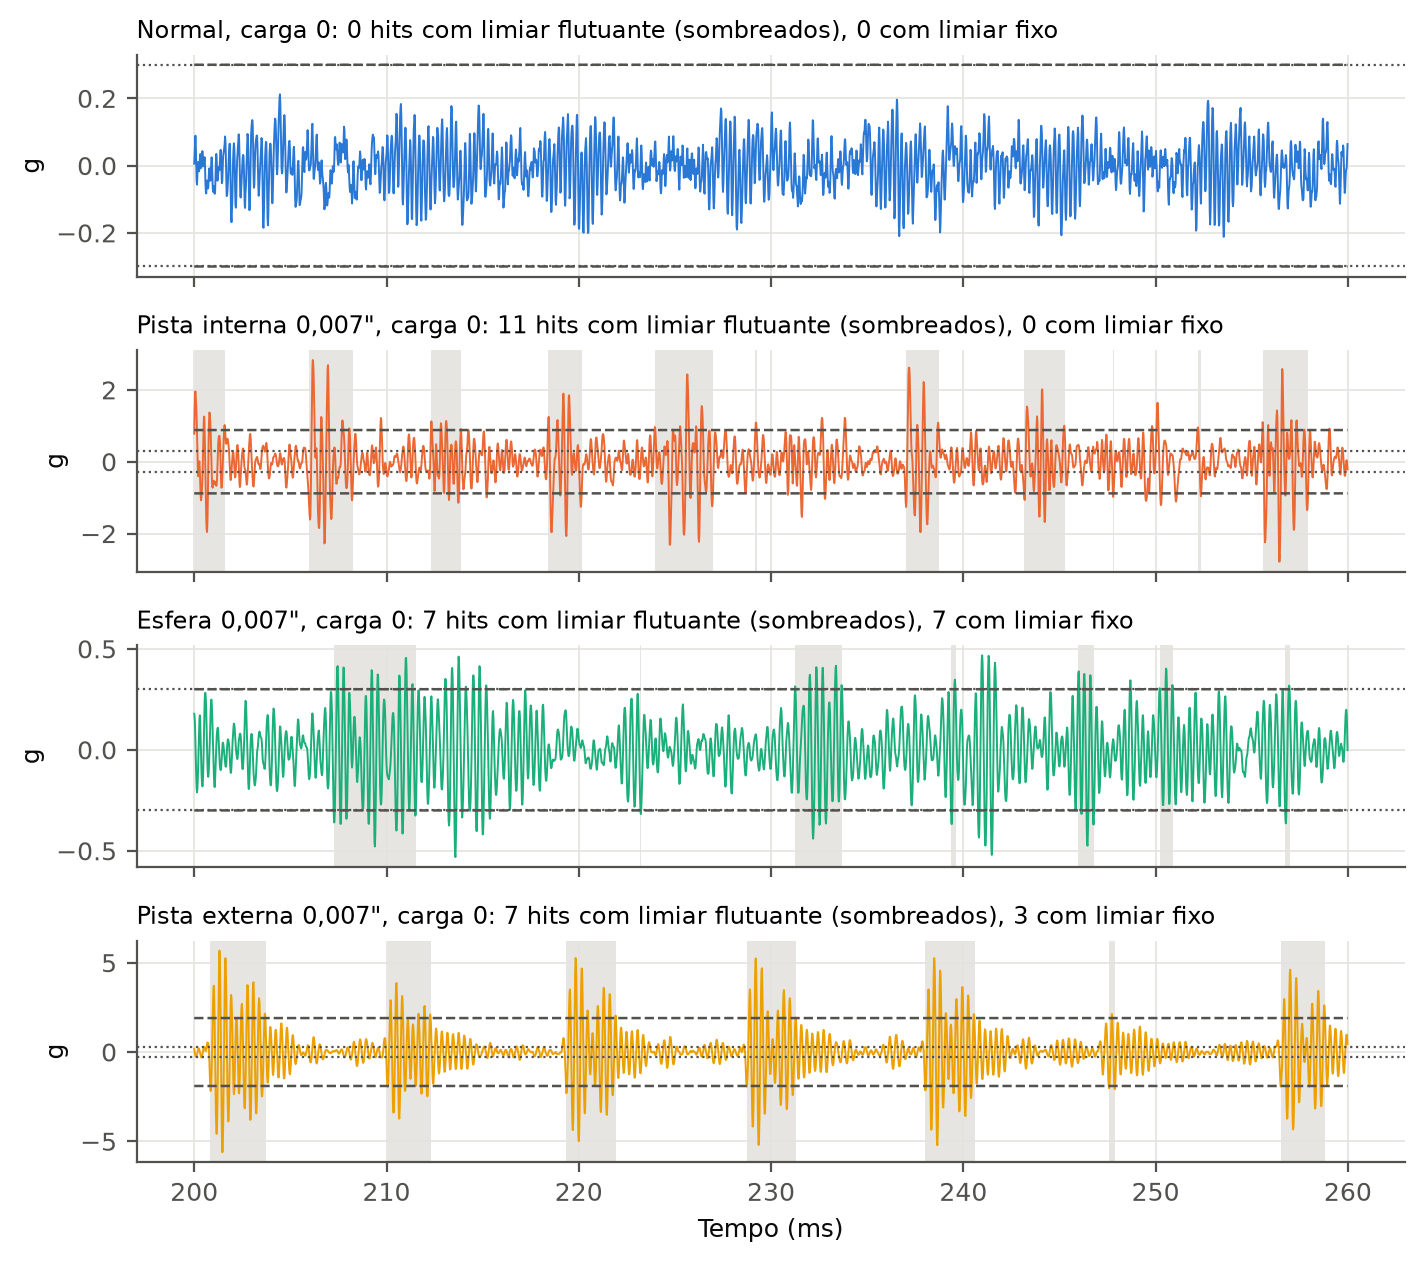
\includegraphics[width=\textwidth]{fig_sinais_hits.png}
	\caption{Trechos de 60\,ms das quatro condições (carga 0, diâmetro de 0,007~polegada). Linhas pontilhadas: limiar fixo de 0,3\,\(g\); tracejadas: limiar flutuante. Áreas sombreadas: \textit{hits} detectados com o limiar flutuante.}
	\label{fig:sinais}
\end{figure}

A Figura~\ref{fig:ordem} mostra a ordem do intervalo entre \textit{hits}. Com limiar fixo, as distribuições são largas e têm picos espúrios perto de 1 e 2, que vêm de \textit{hits} fundidos e truncados. Com limiar flutuante, a pista externa concentra-se em 3,60 (BPFO = 3,58) e a pista interna em 5,27 (BPFI = 5,42); o pequeno desvio da pista interna é compatível com impactos perdidos quando o defeito sai da zona de carga. A esfera fica dispersa em torno de 5,5, longe de 2\(\times\)BSF = 4,71, o que concorda com a dificuldade conhecida de diagnosticar os defeitos de esfera dessa base \cite{smith2015}. Esse descritor é obtido sem FFT, apenas com os instantes dos \textit{hits}, o que reforça a importância do carimbo de tempo de \textit{hardware} ainda pendente no MOMEA.

\begin{figure}[htbp]
	\centering
	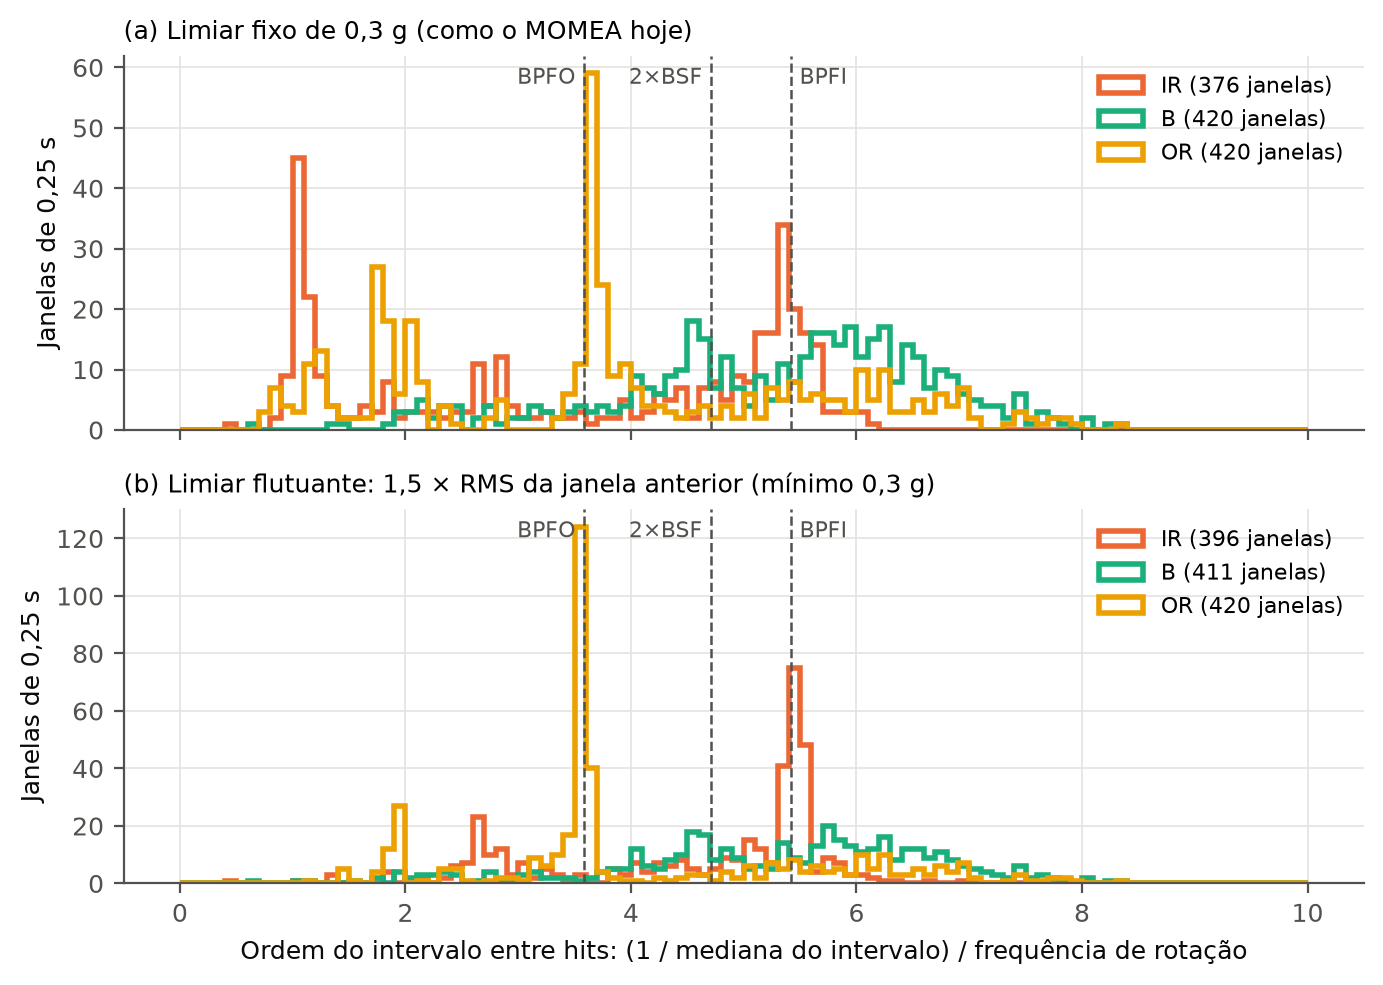
\includegraphics[width=\textwidth]{fig_ordem_ihi.png}
	\caption{Ordem do intervalo entre \textit{hits} por janela, (a) com limiar fixo e (b) com limiar flutuante. Linhas tracejadas: frequências de defeito teóricas em múltiplos da rotação.}
	\label{fig:ordem}
\end{figure}

\subsection{A acurácia depende da validação}

A Figura~\ref{fig:acuracia} e a Tabela~\ref{tab:acuracia} resumem a classificação em quatro classes. Com janelas sorteadas, todos os grupos chegaram a 87--92\,\%, e as diferenças entre eles são pequenas. Deixar uma carga de fora quase não mudou o quadro (82--90\,\%), o que, à primeira vista, sugeriria boa generalização. Não é o caso: o teste ainda contém os mesmos rolamentos físicos, gravados em outra carga.

Quando o diâmetro inteiro sai do treino, a acurácia cai para perto do acaso nos descritores de amplitude: 21\,\% para os clássicos e 25\,\% para os \textit{hits} com limiar fixo, com a MLP. Os \textit{hits} com limiar flutuante sustentaram 46\,\% (53\,\% com RF), e o envelope, que mede diretamente as frequências de defeito, 63\,\%. Juntar todos os descritores não ajudou a MLP (41\,\%): os descritores de amplitude dominam o ajuste e não se transferem entre rolamentos, porque a severidade não é monotônica. Por exemplo, o defeito de 0,014~polegada na pista externa tem RMS de 4 a 8 vezes menor que os de 0,007 e 0,021. Na tarefa de dez classes, a queda das janelas sorteadas para a carga de fora foi um pouco maior (por exemplo, de 91 para 87\,\% com todos os descritores).

\begin{figure}[htbp]
	\centering
	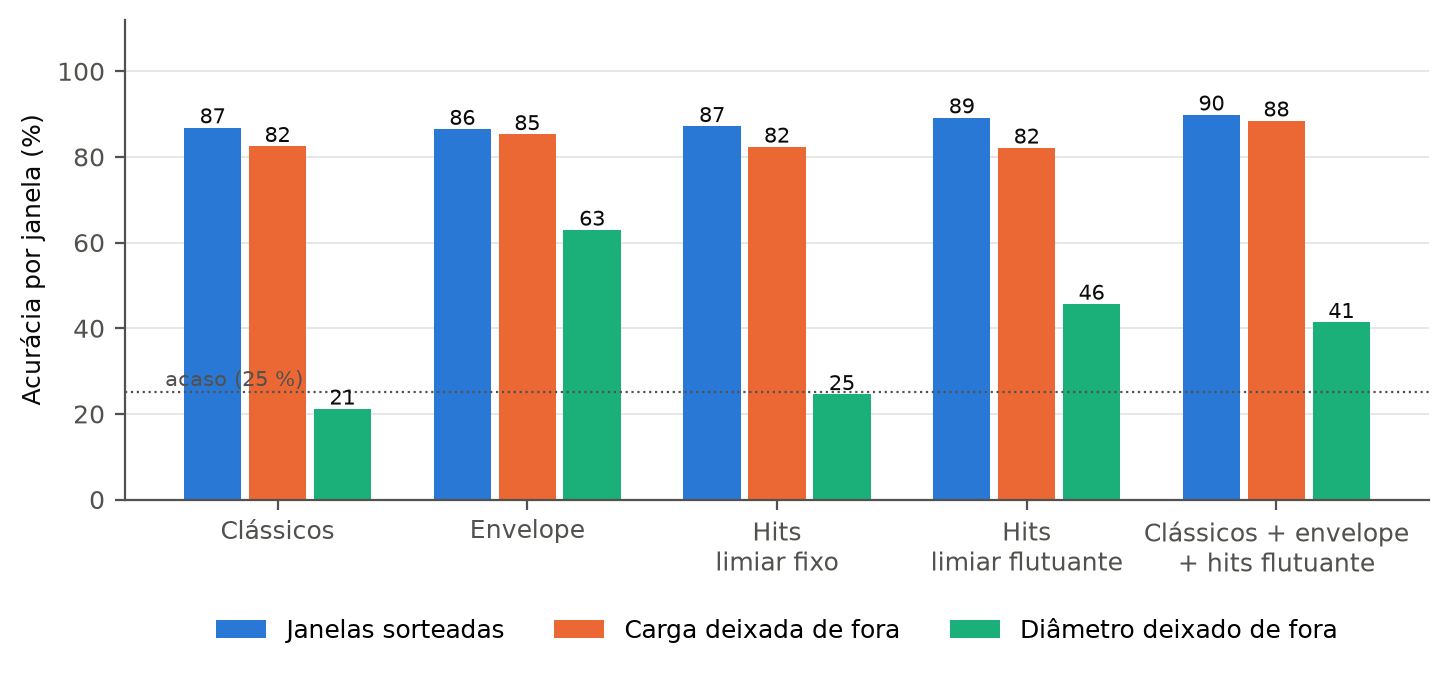
\includegraphics[width=\textwidth]{fig_acuracia_validacoes.png}
	\caption{Acurácia por janela da MLP em quatro classes, por grupo de descritores e validação. A linha pontilhada marca o acaso (25\,\%).}
	\label{fig:acuracia}
\end{figure}

\begin{table}[htbp]
	\centering
	\small
	\caption{Acurácia por janela em quatro classes (entre parênteses, por gravação, com voto majoritário).}
	\label{tab:acuracia}
	\begin{tabular}{llccc}
		\toprule
		\textbf{Descritores} & \textbf{Modelo} & \textbf{Sorteada} & \textbf{Carga de fora} & \textbf{Diâmetro de fora} \\
		\midrule
		Clássicos & MLP & 86,8 (87,5) & 82,5 (82,5) & 21,2 (25,6) \\
		 & RF & 89,5 (92,5) & 86,4 (87,5) & 28,4 (28,2) \\
		Envelope & MLP & 86,5 (90,0) & 85,2 (90,0) & \textbf{62,9} (66,7) \\
		 & RF & 87,4 (90,0) & 85,8 (90,0) & 58,0 (59,0) \\
		\textit{Hits}, limiar fixo & MLP & 87,1 (90,0) & 82,3 (85,0) & 24,6 (20,5) \\
		 & RF & 88,7 (95,0) & 84,4 (80,0) & 35,3 (38,5) \\
		\textit{Hits}, limiar flutuante & MLP & 89,2 (92,5) & 82,1 (82,5) & 45,7 (43,6) \\
		 & RF & 90,5 (92,5) & 87,9 (90,0) & 53,3 (51,3) \\
		Todos (flutuante) & MLP & 89,8 (90,0) & 88,4 (87,5) & 41,4 (38,5) \\
		 & RF & 91,9 (90,0) & 89,6 (87,5) & 54,3 (51,3) \\
		\bottomrule
	\end{tabular}
\end{table}

A Figura~\ref{fig:confusao} mostra onde os erros se concentram, para os \textit{hits} com limiar flutuante. A máquina sã é sempre reconhecida, porque não gera \textit{hits}; o problema está em distinguir os defeitos entre si. Com o diâmetro de fora, a pista externa é confundida principalmente com a interna, e a esfera se divide entre as três classes de defeito.

\begin{figure}[htbp]
	\centering
	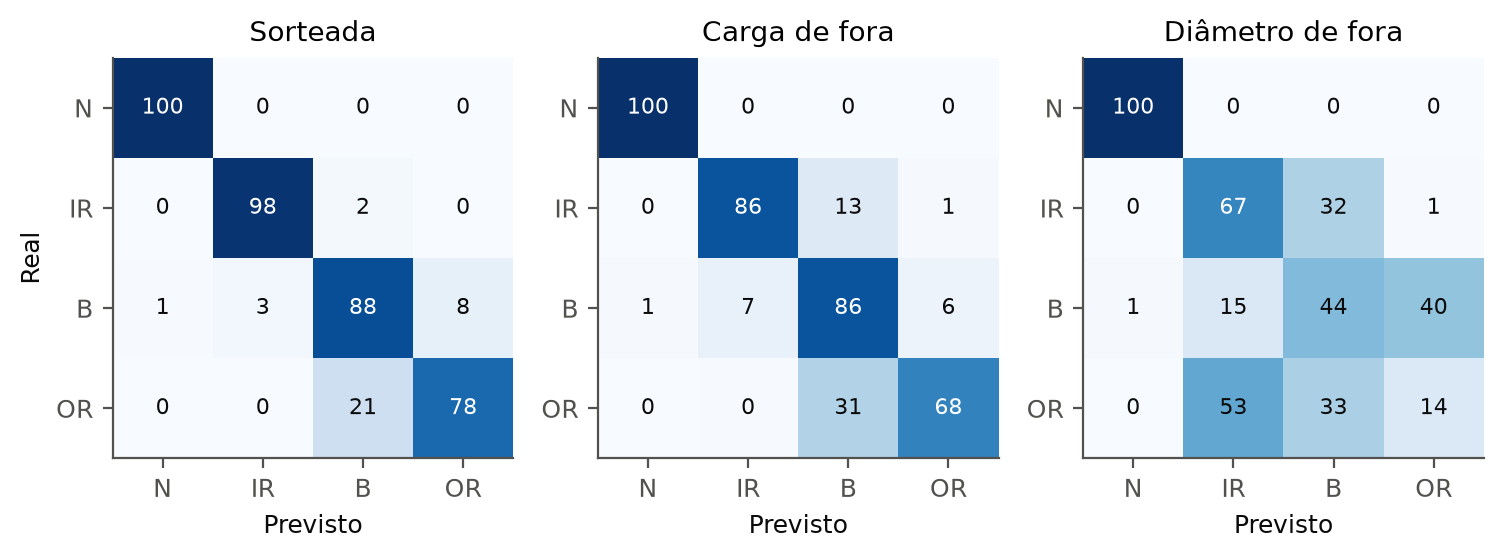
\includegraphics[width=\textwidth]{fig_confusao_hits.png}
	\caption{Matrizes de confusão (\% por linha) da MLP com descritores de \textit{hits} e limiar flutuante, nas três validações.}
	\label{fig:confusao}
\end{figure}

\subsection{MLP int8}

Em cada parte da validação por carga, a MLP treinada foi quantizada para int8 com a mesma aritmética da implementação embarcada \cite{simembarcado2026}: escala de entrada fixa, pesos simétricos por camada e requantização inteira, com escalas calibradas apenas no treino da parte. A Tabela~\ref{tab:int8} mostra que a decisão int8 coincidiu com a de ponto flutuante em 98,4 a 100\,\% das janelas, e que a acurácia mudou no máximo 0,5 ponto percentual.

\begin{table}[htbp]
	\centering
	\small
	\caption{MLP em ponto flutuante e em int8 na validação por carga (quatro classes; faixas sobre as quatro partes).}
	\label{tab:int8}
	\setlength{\tabcolsep}{4pt}
	\begin{tabular}{lccccc}
		\toprule
		\textbf{Descritores} & \textbf{Entradas} & \textbf{MACs} & \textbf{Acc. float} & \textbf{Acc. int8} & \textbf{Concordância} \\
		\midrule
		\textit{Hits}, limiar flutuante & 14 & 3\,072 & 74,3--88,5\,\% & 73,8--88,2\,\% & 99,5--99,7\,\% \\
		Todos & 29 & 4\,032 & 86,5--90,5\,\% & 86,0--90,5\,\% & 98,4--100\,\% \\
		\bottomrule
	\end{tabular}
\end{table}

\subsection{Custo embarcado}

Os custos a seguir são estimativas derivadas dos ciclos medidos na simulação RTL da MicroBlaze a 100\,MHz \cite{simembarcado2026}, e não medições específicas para esta base:
\begin{itemize}
	\item \textbf{detecção dos \textit{hits}}: na lógica, como no MOMEA. A 48\,kHz, o detector é trivial para o FPGA;
	\item \textbf{descritores de \textit{hits}}: o custo medido foi de 4\,232 ciclos por \textit{hit} com FPU e 38\,287 sem. Na maior taxa observada (178 \textit{hits}/s), isso dá cerca de 0,8\,\% e 6,8\,\% da CPU, respectivamente;
	\item \textbf{MLP int8 com 14 entradas}: 3\,072 multiplicações-acumulações, ou cerca de 48 mil ciclos por janela (15,5 ciclos por operação, medidos), isto é, 0,5\,ms a cada 0,25\,s, ou 0,2\,\% da CPU;
	\item \textbf{envelope}: exige filtragem, transformada de Hilbert e FFT por janela. Com \(N = 16\,384\) pontos, cada FFT complexa custa cerca de \(5N\log_2 N \approx 1{,}1\) milhão de operações de ponto flutuante, e são necessárias pelo menos três. Isso dá da ordem de 3 a 4 milhões de operações por janela, ou 12 a 16 milhões por segundo. É inviável na MicroBlaze sem FPU e exigiria um núcleo de FFT na lógica.
\end{itemize}
Há, portanto, um compromisso claro: o envelope generaliza melhor entre rolamentos, mas custa uma FFT por janela; os \textit{hits} com limiar flutuante ficam a meio caminho, por uma fração do custo, e cabem na arquitetura atual do MOMEA.

% =======================================================================================================
\section{Discussão}
\label{sec:discussao}

\subsection{O que este estudo acrescenta à dissertação}

Os resultados reproduzem, numa base pública, as duas lições do estudo da bomba.
\begin{itemize}
	\item \textbf{A validação precisa separar as unidades físicas.} Janelas sorteadas e até cargas deixadas de fora deram 82--92\,\% com qualquer grupo de descritores, porque o modelo reconhece o rolamento, e não o tipo de defeito. Só separando os rolamentos a diferença entre os descritores aparece. É o mesmo padrão do LORO na bomba, em que a configuração das válvulas caiu de 89--95\,\% para 21--28\,\%. Na CWRU, porém, sabe-se que os defeitos são reais e localizados, de modo que a queda não pode ser atribuída à falta de efeito físico; ela vem da pouca diversidade de unidades (nove rolamentos com defeito e um são).
	\item \textbf{O limiar fixo do extrator falha diante de emissão contínua.} Com limiar fixo, os impactos se fundiram e foram truncados pela duração máxima, e os descritores de \textit{hits} ficaram no acaso fora da amostra. Com um limiar flutuante, os \textit{hits} recuperaram a periodicidade do defeito e a acurácia quase dobrou. Isso dá uma recomendação concreta para o MOMEA: oferecer um limiar flutuante na lógica, junto com a revisão do ganho já indicada pelos ensaios da bomba.
\end{itemize}

\subsection{Limitações}

\begin{itemize}
	\item Os sinais são de vibração, a 48\,kHz; nem os descritores nem as conclusões se transferem diretamente para EA de alta frequência ou para cavitação.
	\item O fator do limiar flutuante e o DDT foram escolhidos com base na concordância com as frequências de defeito, o que usa os rótulos; o ganho na validação por diâmetro pode estar ligeiramente otimista.
	\item Há apenas três partes na validação por diâmetro e nove rolamentos com defeito, de modo que as acurácias fora da amostra têm grande incerteza.
	\item Os defeitos são artificiais (eletroerosão) e únicos por condição; algumas gravações são atípicas, e os defeitos de esfera dessa base são sabidamente difíceis \cite{smith2015}.
	\item Os custos embarcados são estimativas a partir de medições em outra cadeia; o caminho completo para esta base não foi simulado em RTL.
\end{itemize}

% =======================================================================================================
\section{Conclusões}
\label{sec:conclusoes}

Aplicado à base CWRU, o fluxo desenvolvido para o MOMEA mostrou que descritores de \textit{hits} capturam a periodicidade dos defeitos de rolamento quando o limiar acompanha o nível do sinal, e que a acurácia relatada depende essencialmente da validação: 87--92\,\% com janelas sorteadas e 21--63\,\% com rolamentos nunca vistos. O envelope foi o grupo que mais generalizou, e os \textit{hits} com limiar flutuante ficaram a meio caminho, por uma fração do custo computacional e compatíveis com a arquitetura embarcada. A MLP int8 preservou a decisão em 98 a 100\,\% das janelas.

Para a dissertação, o estudo serve como validação externa do método e reforça duas recomendações ao MOMEA: implementar um limiar flutuante no extrator e o carimbo de tempo de \textit{hardware}, que viabiliza os descritores de periodicidade. A comparação com outros trabalhos na base CWRU deve ser sempre feita sob o mesmo esquema de validação.

\section*{Reprodutibilidade}

O estudo inteiro é executado por \texttt{CWRU/cwru\_mlp.py} sobre os arquivos em \texttt{CWRU/Dados/}, cuja lista, com endereços e tamanhos, está em \texttt{Dados/lista\_arquivos.json}. As saídas, com janelas, inventário, métricas, int8, figuras e resumo, estão em \texttt{CWRU/resultados/}.

% =======================================================================================================
\begin{thebibliography}{99}

	\bibitem[Autores(2026a)]{mlpbomba2026}
	AUTORES.
	\newblock Classificação das condições de operação de uma bomba por emissão acústica: redes MLP, florestas aleatórias e \textit{gradient boosting} sobre \textit{hits} extraídos em FPGA, com validação por corrida.
	\newblock Relatório técnico, 2026.

	\bibitem[Autores(2026b)]{simembarcado2026}
	AUTORES.
	\newblock Inferência embarcada de redes MLP para emissão acústica em FPGA Artix-7: implementação em MicroBlaze e em lógica dedicada, verificada por simulação.
	\newblock Relatório técnico, 2026.

	\bibitem[CWRU(s.d.)]{cwru}
	CASE WESTERN RESERVE UNIVERSITY.
	\newblock \emph{Bearing Data Center}: 48k Drive End Bearing Fault Data; Normal Baseline Data.
	\newblock Disponível em: \url{https://engineering.case.edu/bearingdatacenter}. Acesso em: 10 nov. 2026.

	\bibitem[Hendriks et al.(2022)]{hendriks2022}
	HENDRIKS, J.; DUMOND, P.; KNOX, D. A.
	\newblock Towards better benchmarking using the CWRU bearing fault dataset.
	\newblock \emph{Mechanical Systems and Signal Processing}, v. 169, 108732, 2022.

	\bibitem[Pedregosa et al.(2011)]{pedregosa2011}
	PEDREGOSA, F. et al.
	\newblock Scikit-learn: machine learning in Python.
	\newblock \emph{Journal of Machine Learning Research}, v. 12, p. 2825--2830, 2011.

	\bibitem[Randall e Antoni(2011)]{randall2011}
	RANDALL, R. B.; ANTONI, J.
	\newblock Rolling element bearing diagnostics---a tutorial.
	\newblock \emph{Mechanical Systems and Signal Processing}, v. 25, n. 2, p. 485--520, 2011.
	\newblock DOI: \href{https://doi.org/10.1016/j.ymssp.2010.07.017}{10.1016/j.ymssp.2010.07.017}.

	\bibitem[Rauber et al.(2021)]{rauber2021}
	RAUBER, T. W.; LOCA, A. L. S.; BOLDT, F. A.; RODRIGUES, A. L.; VAREJÃO, F. M.
	\newblock An experimental methodology to evaluate machine learning methods for fault diagnosis based on vibration signals.
	\newblock \emph{Expert Systems with Applications}, v. 167, 114022, 2021.

	\bibitem[Smith e Randall(2015)]{smith2015}
	SMITH, W. A.; RANDALL, R. B.
	\newblock Rolling element bearing diagnostics using the Case Western Reserve University data: a benchmark study.
	\newblock \emph{Mechanical Systems and Signal Processing}, v. 64--65, p. 100--131, 2015.
	\newblock DOI: \href{https://doi.org/10.1016/j.ymssp.2015.04.021}{10.1016/j.ymssp.2015.04.021}.

	\bibitem[Vallen Systeme(2022)]{vallen2022}
	VALLEN SYSTEME GMBH.
	\newblock \emph{AMSY-6: System Specification}.
	\newblock Wolfratshausen: Vallen Systeme GmbH, 2022.

\end{thebibliography}

\end{document}
